% \AtBeginSection[]{
%     \begin{frame}
%         \frametitle{}
%         \tableofcontents[currentsection]
%     \end{frame}
% }

%%%%%%%%%%%%%%%%%%%%%%%%%%%%%%%%%%%%

\section{AOMEA approach}

\subsection{Overview}

\begin{frame}{AOMEA approach}{Overview}

    \begin{columns}

        \begin{column}{0.5\textwidth}

            \centering
            \vspace{-1ex}
            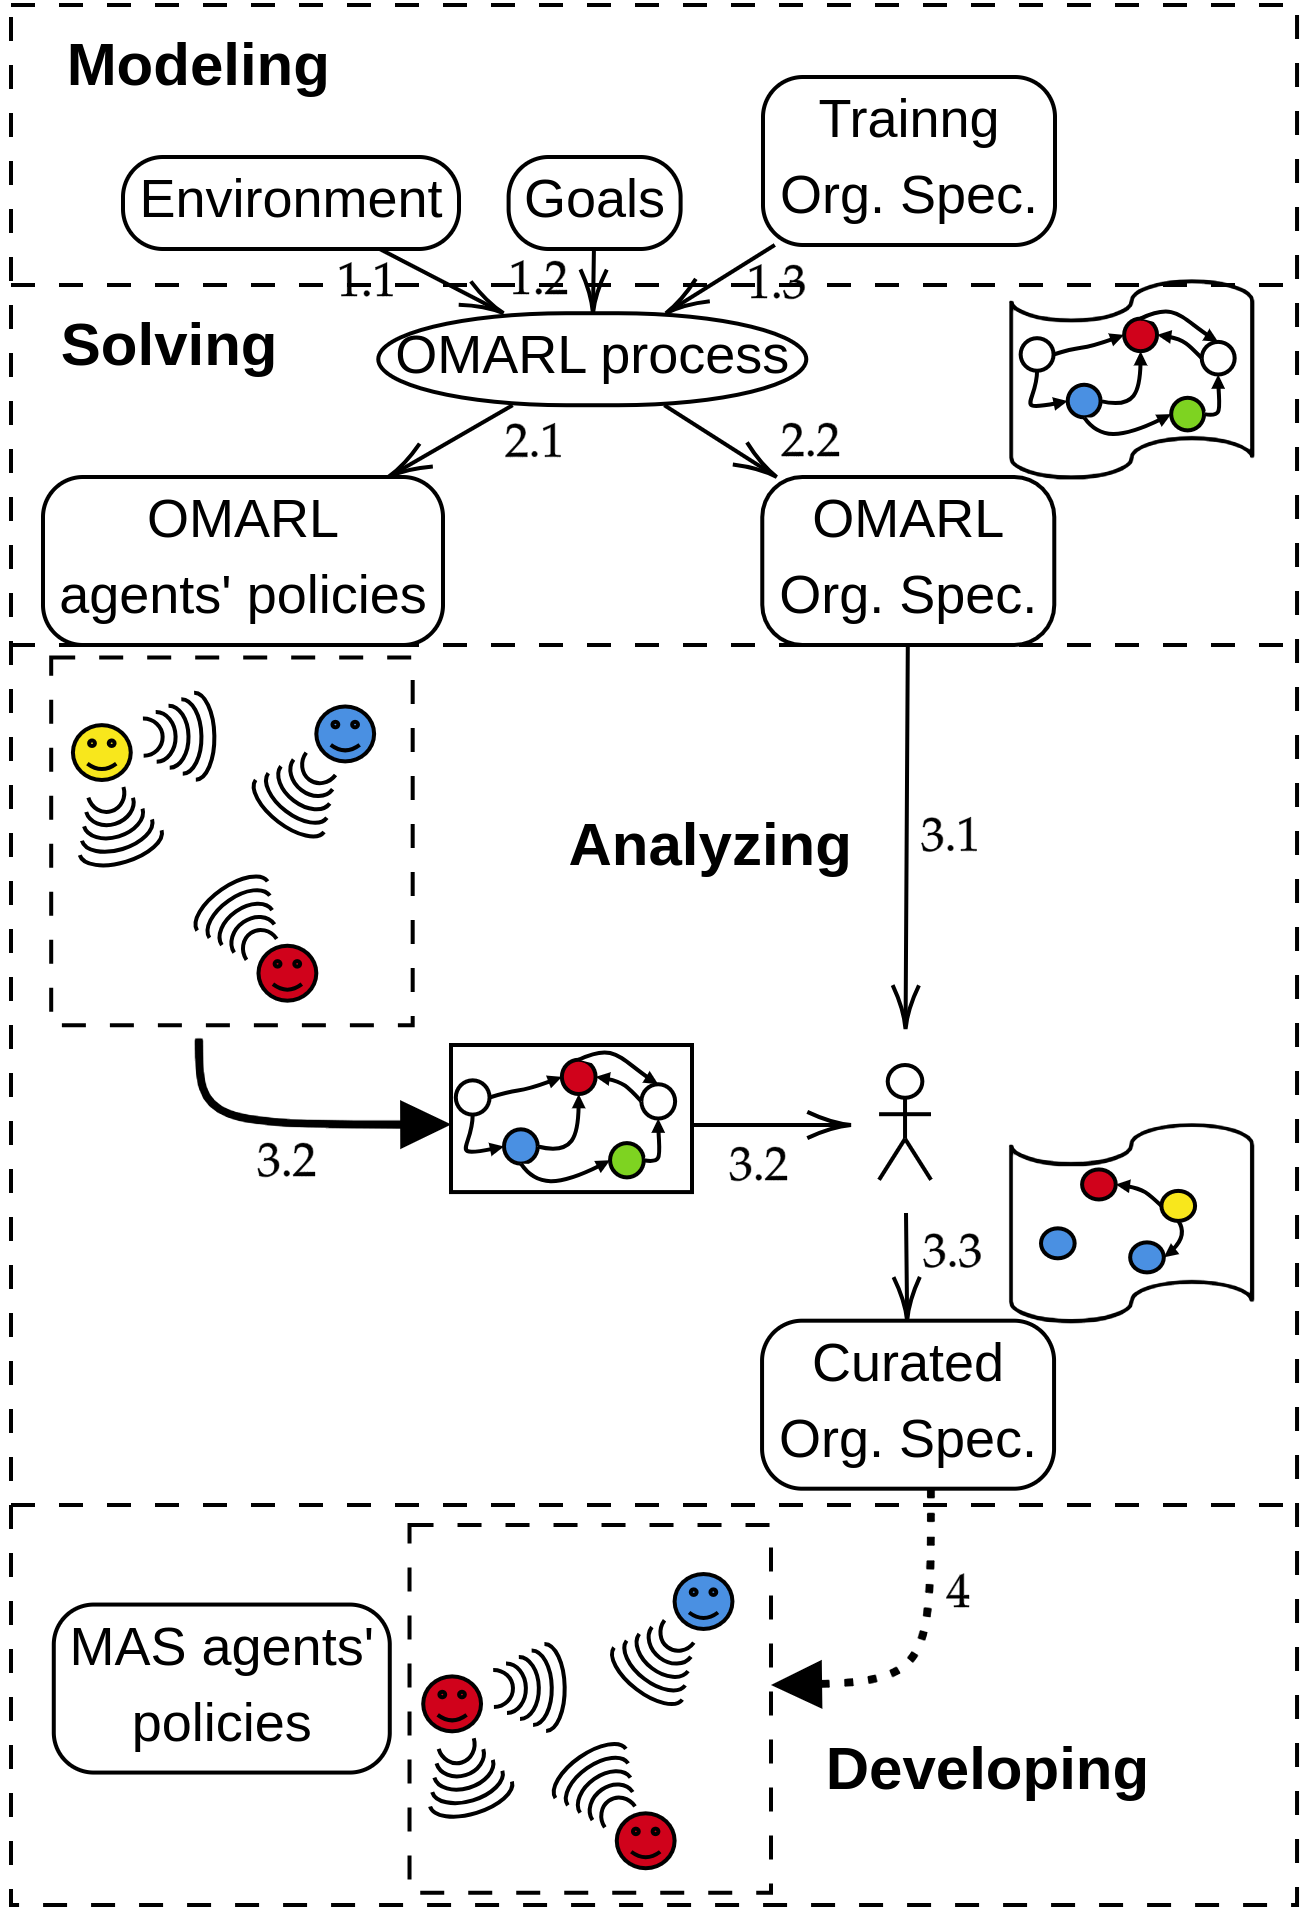
\includegraphics[width=\linewidth]{figures/AOMEA_illustrative_global_view.png}

        \end{column}

        \begin{column}{0.5\textwidth}
            \centering
            \adjustbox{trim={0.\width} {0.56\height} {0.\width} {0.\height}, clip}{%
                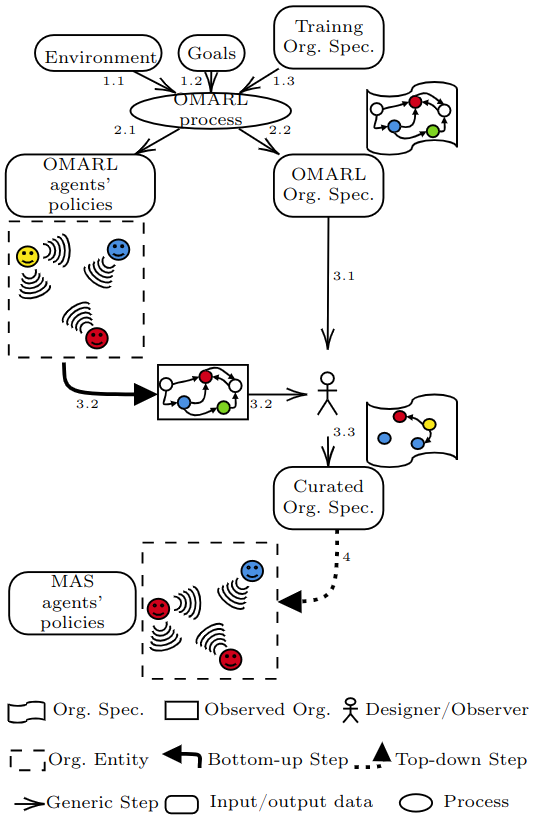
\includegraphics[width=1.2\linewidth]{figures/AOMEA_illustrative_view}
            }
        \end{column}

    \end{columns}

\end{frame}


\subsection{Engineering tool}

\begin{frame}[fragile]{AOMEA approach}{Engineering tool}

    \begin{block}{\emph{PRAHOM PettingZoo Wrapper}\label{PettingZoo-wrapper}}
        \begin{itemize}
            \item Uses \textbf{PettingZoo}: a library with a standardized API that facilitates the application of MARL algorithms;
            \item Proposed as a tool to help the application of \emph{PRAHOM} for a given PettingZoo environment.
        \end{itemize}
    \end{block}

    \

    \begin{lstlisting}[language=Python, caption=PRAHOM PettingZoo Wrapper basic use, label={lst:wrapper_basic_use}]
    from omarl_experiments import prahom_wrapper
    env=PettingZoo_env.parallel_env(render_mode="human")
    specs_to_hist={"structural_specifications":{"roles":{"follower":{"23":41,"14":[74,0]}}...},"functional_specifications":{"links":{"(leader,follower,aut)":".*14.*?89"}...}...}
    policy_specs_constr={"agent_0":{"structural_specifications":"roles":["follower"]}}
    env=prahom_wrapper(env,action_to_specs,training_specs)
    env.train("default_PPO")
    trained_specs,agent_to_specs=env.prahom_specs()
    \end{lstlisting}

\end{frame}
